\section{Theorie}
\label{sec:Theorie}

In diesem Versuch geht es um die Messung von ionisierender Strahlung durch 
das Geiger-Müller Zählrohr, dessen Funktionsweise noch in Folgenden
erläutert wird. Unter genannten Strahlung fallen zahlreiche
Strahlungstypen, vor Allem $\alpha-, \beta-$ und $\gamma$-Strahlung. Im 
Allgemeinen sind das He-Kerne ($\alpha$), Elektronen ($\beta^-$) oder Positronen
($\beta^+$) sowie letztlich elektromagnetische Strahlung ($\gamma$). Hier geht
es überwiegend um die ersten beiden Typen, da es mithilfe des Geiger-
Müller Zählrohrs aufgrund der geringen Intensität schwierig ist, letzteres
nachzuweisen.
\vspace{0.5em}
\\
\noindent Das Geiger-Müller-Zählrohr besteht aus einem Kathodenzylinder und 
einem Anodendraht im Zentrum. Dieser ist positiv geladen, der Zylinder hingegen 
negativ und beinhaltet ein Edelgas. $\beta$-Strahlung, welche durch das dünne 
Glas der Röhre fliegt, trifft auf die Atome im Inneren und Schlägt ein Elektron 
aus der Hülle heraus; es kommt zur Ionisation. Das Elektron fliegt in Richtung 
Anodendraht, während das Atom in Richtung Zylinder abdriftet, die hingegen 
positiv geladenen Edelgasatome bewegen sich an den negativ geladenen Rand des 
Rohres um sich zu neutralisieren.
\vspace{0.5em}
\\
\noindent Dieser Prozess lässt sich in verschiedene 
Phasen unterteilen, angefangen mit der Rekombination. In dieser Phase kommt es 
zu ersten Ionsationen, allerdings ist das elektrische Feld so schwach, dass 
die Elektronen und Ionen sofort wieder rekombinieren bevor sie die Kathode und 
Anode erreichen. Mit zunehmender Spannung nimmt die Anzahl an Neutralisierungen 
dementsprechend ab.
\vspace{0.5em}
\\
\noindent Als nächstes kommt es zur Ionisationskammer. Die Betriebsspannung ist 
inzwischen so groß, dass alle Elektronen die Anode erreichen, welche durch
die Primärstrahlung erzeugt wurden. Es entsteht eine Proportionalität zwischen 
Ionisationsstrom und Energie.
\vspace{0.5em}
\\
\noindent Anschließend folgt der Proportionalitätsbereich. Bei weiterer Erhöhung 
der Spannung kommt es zu zusätzlichen Stoßprozessen, welche zu einer erhöhten 
Intensität führen. Die Elektronen werden so stark beschleunigt, dass sie durch 
Stoßionsiationen weitere Ionenpaare erzeugen. Dieser Effekt wird als Townsend-
Lawine bezeichnet, da die Elektronen wie eine Lawine für weitere Stöße sorgen.
Es kommt zu einer Ionisationskettenreaktion, welche jedoch örtlich begrenzt ist;
in der Nähe des Anodendrahtes ist ein Verstärkungsfaktor von $10^3$ festzustellen.
\vspace{0.5em}
\\
\noindent Das nächste Segment wird als Geiger-Müller-Bereich bezeichnet. Hier
ist die Intensität wiederum höher als im Bereich davor, da sich die Entladungen
unkontrolliert über das gesamte Zählrohr ausbreiten. Ursache ist die extreme
Gasverstärkung: Durch Stöße angeregte Gasatome emittieren UV-Photonen, die an
der Kathode weitere Elektronen auslösen und den Lawineneffekt verstärken.
Diese Rückkopplung führt dazu, dass jedes einfallende Teilchen, unabhängig
von seiner Energie, eine maximale Entladung auslöst. Dadurch entsteht das
charakteristische Geiger-Müller-Plateau: Über einen weiten Spannungsbereich 
bleibt die Zählrate nahezu konstant, da die Signalhöhe stets gesättigt ist.
Allerdings setzen sich trägere Atomrümpfe setzen sich am Draht ab und bilden
eine positive Ladungswolke, welche das elektrische Feld lokal abschirmt. Als
Präventativmaßnahme kann Alkohol hinzugefügt werden. Dieser hat den Zweck, die
Photonen zu absorbieren und demzufolge das Auslösen weiterer Elektronen zu
verhindern.
\vspace{0.5em}
\\
\noindent An den Geiger-Müller-Bereich schließt zuletzt die Dauerentladung an.
Wird die Spannung zu hoch geregelt, kann das zu Schäden am Gerät führen.
\vspace{0.5em}
\\
\noindent Eine schematische Darstellung des Ablaufs bei kontinuierlicher 
Spannungsveränderung ist in \autoref{fig:3} dargestellt.
\begin{figure}[H]
    \centering
        \centering
        \includegraphics[width=0.7\textwidth]{Bilder/phasen.png}
        \caption{Phasen im Geiger-Müller-Zählrohr. \cite{anleitung6}}
    \hfill
    \label{fig:3}
\end{figure}

\subsection{Totzeit und Erholungszeit}
Zu dem Zeitpunkt, wo sich die Raumladungswolke um den Anodendraht bildet, kommt 
es zu einem entscheidenden Moment. Nach jeder Detektion eines Teilchens benötigt
das Zählrohr eine gewisse Zeit, um wieder voll funktionsfähig zu sein. Diese
Unterbrechung setzt sich aus zwei Phasen zusammen: der Totzeit und der Erholzeit.
Die Totzeit kommt zustande, indem die positive Ionenwolke das elektrische Feld 
blockiert, sodass der Zähler keine neuen Teilchen detektieren kann. Letzteres 
beschreibt die Zeit, in der die Ionen wieder langsam zur Kathode zurückwandern. 
Das elektrische Feld baut sich wieder auf, erst danach ist die Anode wieder 
empfindlich gegenüber erneuten Empfangs von Elektronen. Für die Bestimmung der 
Totzeit mithilfe des Oszilloskops wird der Abstand der Peaks, wie in \autoref{fig:4}
zu sehen, abgelesen.
\begin{figure}[H]
    \centering
        \centering
        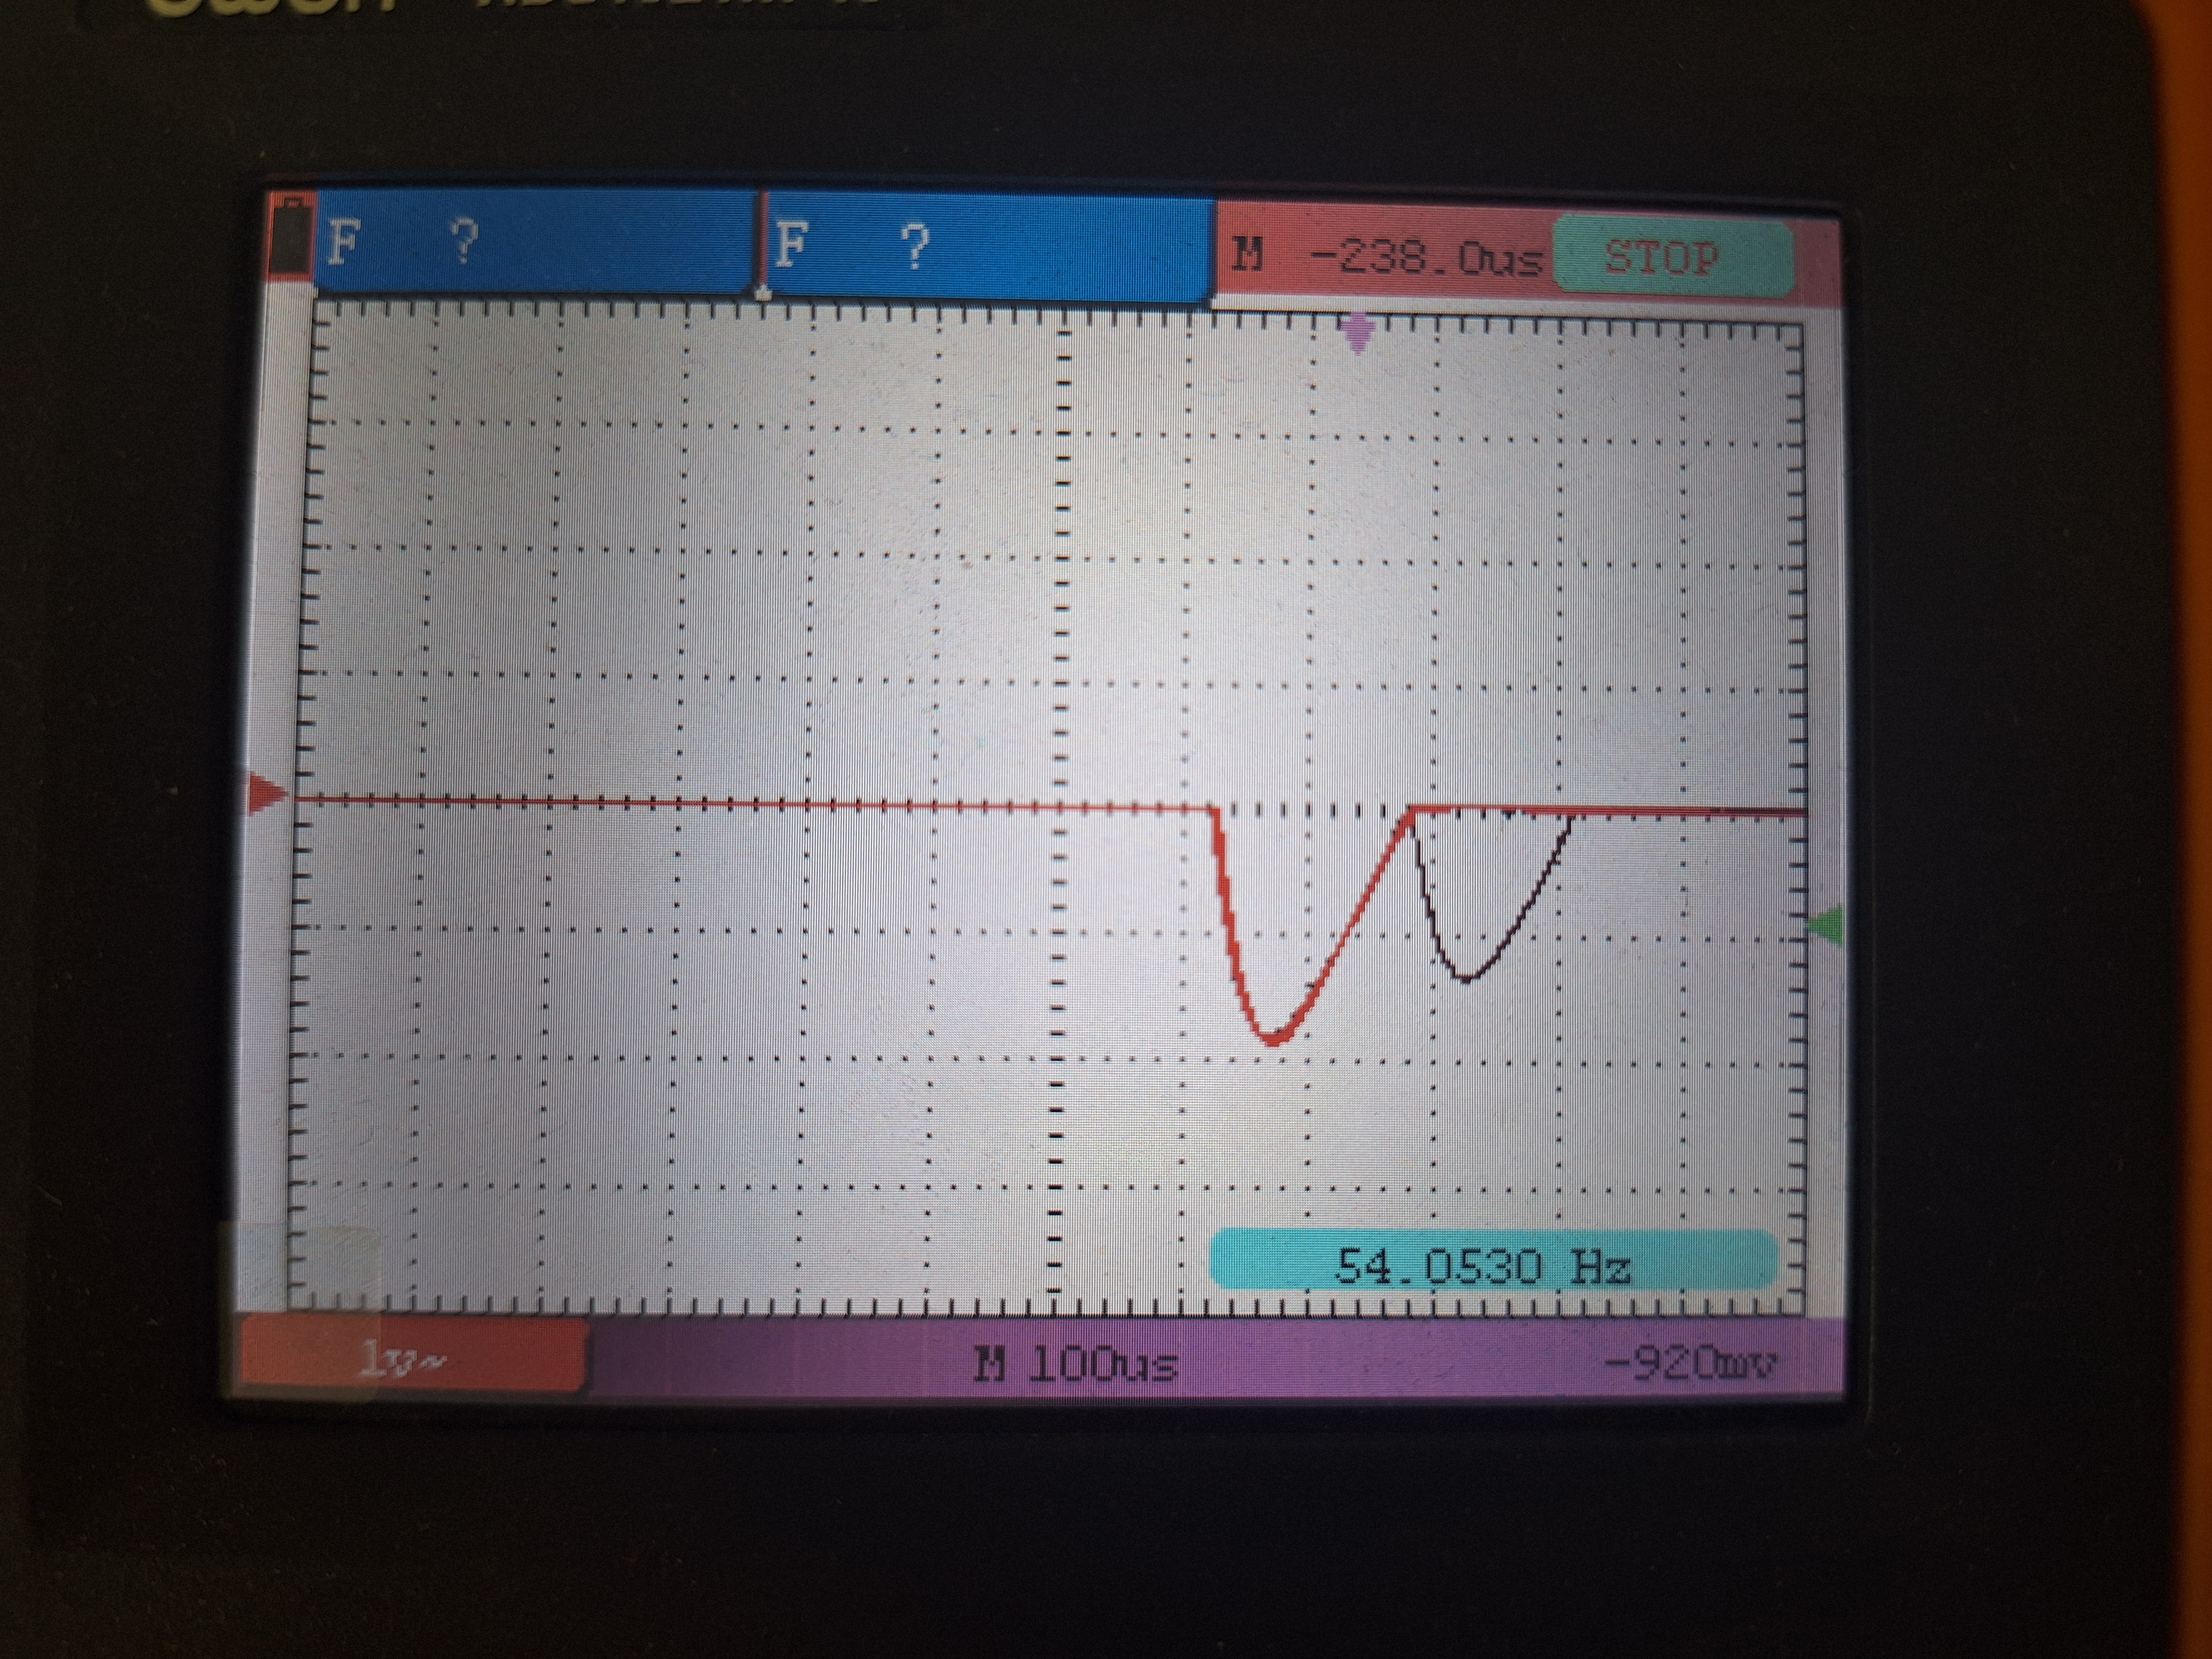
\includegraphics[width=0.7\textwidth]{Bilder/totzeit.jpg}
        \caption{Totzeit am Oszilloskop.}
    \hfill
    \label{fig:3}
\end{figure}
\noindent Für die Zwei-Quellen Methode werden die Zählraten $N_1, N_2$ und 
$N_{12}$ benötigt (wobei $N_1$ für die 1. Quelle, $N_2$ für die 2. Quelle und 
$N_{12}$ für beide Quellen zusammen steht). Für die Totzeit ergibt sich der 
Zusammenhang
\begin{equation}
    \tau = \frac{N_1 + N_2 - N_{12}}{N_{12}^2 - N_1^2 -N_2^2}.
\end{equation}

\subsection{Güte des Zählrohrs}
Sofern energiereiche Elektronen auf die Kathode treffen und dort sekundäre 
Elektronen auslösen, so können diese die Anode erreichen und dort einen 
weiteren Impuls auslösen. Dieser Effekt wird als Nachentladung bezeichnet und 
lässt sich durch Löschgas in Form des vorherigen angesprochenen Alkohol 
herunterregeln, indem die Moleküle die Energie der Ionen durch Stöße absorbieren.
Je besser das Löschgas, desto geringer ist die Steigung des Geiger-Müller-Plateaus, 
im Idealfall liegt diese also bei 0. Die Steigung des Plateaus kann als Maß 
für die Güte herangezogen werden. Für diese gilt die Gleichung 
\begin{align}
    s &= \frac{\increment N}{N} \cdot \frac{100\%}{100V}.\\
      &= s = \frac{z\left(U_\text{A} + 50\unit{\volt}\right) - z\left(U_\text{A} - 50\unit{\volt}\right)}{z \cdot U_\text{A}} \cdot \frac{100\%}{100\unit{\volt}}
\end{align} 

\subsection{Fehlerrechnung}
Die gemessenen Werte unterliegen Messunsicherheiten und werden demnach im
Folgenden nicht als fehlerfrei angesehen. Die Fehler entstehen bei der
Bildung der Mittelwerte durch den Fehler des Mittelwerts und bei der
Regressionsrechnung sowie der Fehlerforpflanzung durch Python.
Der Mittelwert ist definiert durch
\begin{equation}
    \overline{x} = \frac{1}{N} \sum\limits_{i=1}^N x_i.
\end{equation}
\noindent Der Fehler des Mittelwerts ist somit gegeben durch 
\begin{equation}
    \begin{aligned}
        \increment \overline{x} &= \sqrt{\overline{x^2\kern-0.1em} - \overline{x}^2} \\
                            &= \frac{\sqrt{\frac{1}{N-1} \sum\limits_{i=1}^N (x_i - \overline{x})^2}}{\sqrt{N}}.
    \end{aligned}
\end{equation}

Um Fehler einzubeziehen, wird die Gauß'sche Fehlerfortpflanzung verwendet:
\begin{equation}
    \label{eqn:9}
    \increment f = \sqrt{\left(\frac{\partial f}{\partial x}\right)^2 \cdot \left(\increment x\right)^2 + \left(\frac{\partial f}{\partial y}\right)^2 \cdot \left(\increment y\right)^2 + .... + \left(\frac{\partial f}{\partial z}\right)^2 \cdot \left(\increment z\right)^2}
\end{equation}